\documentclass[../main.tex]{subfiles}
\graphicspath{{\subfix{../images/}}}
\begin{document}
	
	\chapter{Introduction and motivations}
	
	This work is a scientific study of photodetectors used in astronomical space missions. In particular, the work aims to study and characterize a \textbf{photosensitive detector} for use in \textbf{astrophotometry}. The focus will be on the proposed astronomical space mission \textbf{ST}ars and \textbf{E}xo\textbf{P}lanets (\textbf{STEP}), which has been placed on the National Roadmap for Research Infrastructure \cite{stepprodex}. STEP is proposed as a micro-satellite mission, that will study stars and exoplanets by supplying chromatic observations of star fluxes using a \textbf{charge-coupled device (CCD)} detector. A CCD is a kind of photosensitive detector, and this detector type will be the focus of the following work. This mission proposal, in its initial form, will be the starting point of this work. This will be subject to change, and recent cuts in funding may result in smaller changes to the scientific goals of the mission. All of this serves to illuminate the difficult processes involved with planning space missions, and conducting initial feasibility tests. 
	
	The goal is to develop a testing procedure that enables technical requirements to be output from mission requirements that arise from the scientific goals. Two such requirements are of significance for the payload. These requirements are the construction of a precise \textbf{linearity curve} of the CCD response, and a determination of constraints on the \textbf{pointing precision} (attitude requirement) of the satellite. They are explained in detail below. The main focus will be on these two top-level mission requirements and their consequences for the technical requirements. 
	
	We shall begin in this chapter, with an introduction to the motivations behind this study. This is achieved through a cursory outline of the science case. A historical perspective on satellite missions is given first, followed by an outline of the relevant exoplanet science needed to understand the following line of work. The initial mission design for STEP will be presented, and the mission requirements will be deduced and explained thoroughly. 
	
	Throughout the work, the focus of the study will be the goal of exoplanet detection via the transit method.  STEP will also supply data for stellar research, but the constraints posed on the system, arising from the goal of planetary detection is the limiting factor.

	\section{Small satellites}
	STEP is an astronomical \textbf{microsatellite} mission. A microsatellite is, in short terms, a small satellite, usually with a mass below $100$ kg\cite{SSE}, although this definition varies wildly. They are typically inexpensive and small in comparison to conventional satellites - usually around 1/10th or 1/100th, of the mass and cost of a conventional satellite \cite{SSE}. 
	\begin{figure}[H]
		\centering			
		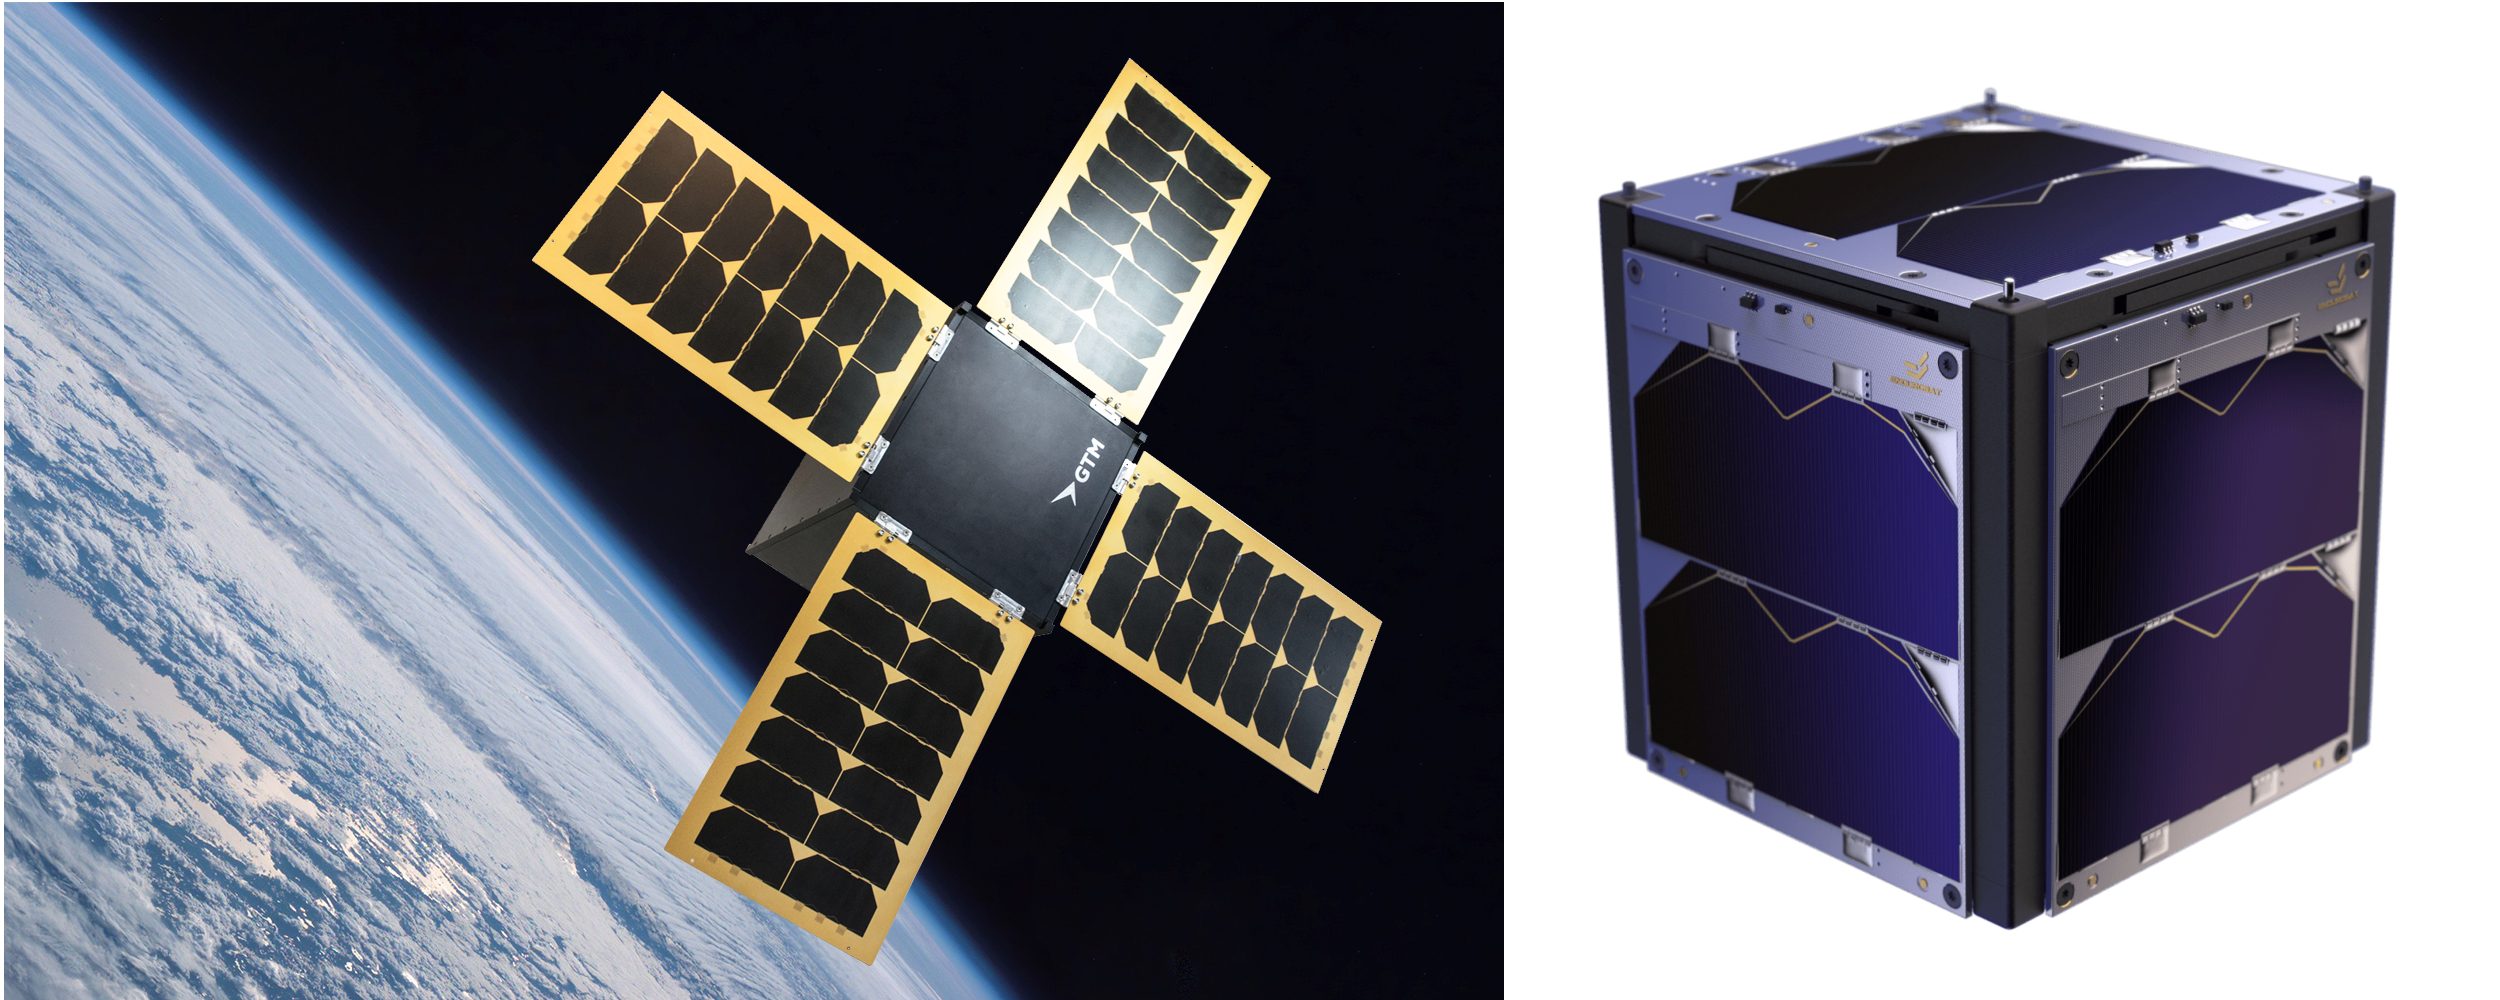
\includegraphics[width=1\textwidth]{cubesats.png}
		\caption{\textbf{Left:} A 12U cubesat in space, with expanded solar panels\cite{cubesatimage}. \textbf{Right:} An example of a $10\text{cm} \times 10\text{cm} \times 10$ cm 1U cubesat unit. Solar panels are mounted on the side for power supply. }
		\label{fig:cubesatex}
	\end{figure}
	
	The first western satellites were small out of necessity \cite{SSE}. The demand for larger and more complex satellites grew, limiting space to a few nations. This was mostly due to the need for bigger and more complex launchers. However, advances in very large-scale integration (VLSI), enabled complex electrical systems to be built small without large demands on power. This led to the development of the microsatellite. Several flights of microsatellites were achieved in the 70s \cite{SSE}, and in 1981 students and staff at the University of Surrey had developed a microsatellite, \textbf{UoSAT-1}, that was launched by NASA \cite{uosat}. 
	
	The development and usage of small satellites have seen a considerable boost with the introduction of the \textbf{CubeSat}. A CubeSat is a small, 1kg, satellite of dimensions $10\text{cm} \times 10\text{cm} \times 10$ cm. This is referred to as a 1U unit CubeSat and was first proposed by Professor Robert Twiggs of Stanford university's Space Systems Development Laboratory \cite{SSE, cubesatref}. Such a 1U satellite is seen in figure \ref{fig:cubesatex}. These units may be combined to build larger satellites, enabling bigger and more complex configurations.  
	
	This small satellite revolution makes missions like STEP possible, as financing and infrastructure would otherwise inhibit possibilities in space for a small nation such as Denmark. The advancements in small satellites enable students and young scientists to get hands-on experience with every aspect of space mission development.
	
	\section{Exoplanets}
	STEP is to detect exoplanets and measure their size. An extrasolar planetary body (exoplanet), is a planet in orbit around a star that is not our sun. The search for exoplanets has long been of interest within the astrophysical community. The discovery of the first exoplanet in 1995 \cite{firstexoplanet} marked the beginning of a new fundamental field of science. Since then, an extensive catalog of exoplanets of various types has been constructed, and the field has matured. 
	
	The search for habitable exoplanets is of particular interest, as it is linked to our fundamental existential curiosity about the potential of life on distant worlds. Recently many potentially habitable exoplanets have been discovered, but the question of habitability beyond determining whether the planet is situated within the so-called \textbf{habitable zone}\footnote{The habitable zone is defined as the range of orbital distances of a planet from its parent star, at which liquid water can exist on the surface\cite{habitablezone}.}, has been difficult to address \cite{stepprodex}. 
	These questions relate to the composition of the planet itself and its atmosphere, and the STEP mission will address these questions. 
	\begin{figure}[hb!]
		\centering			
		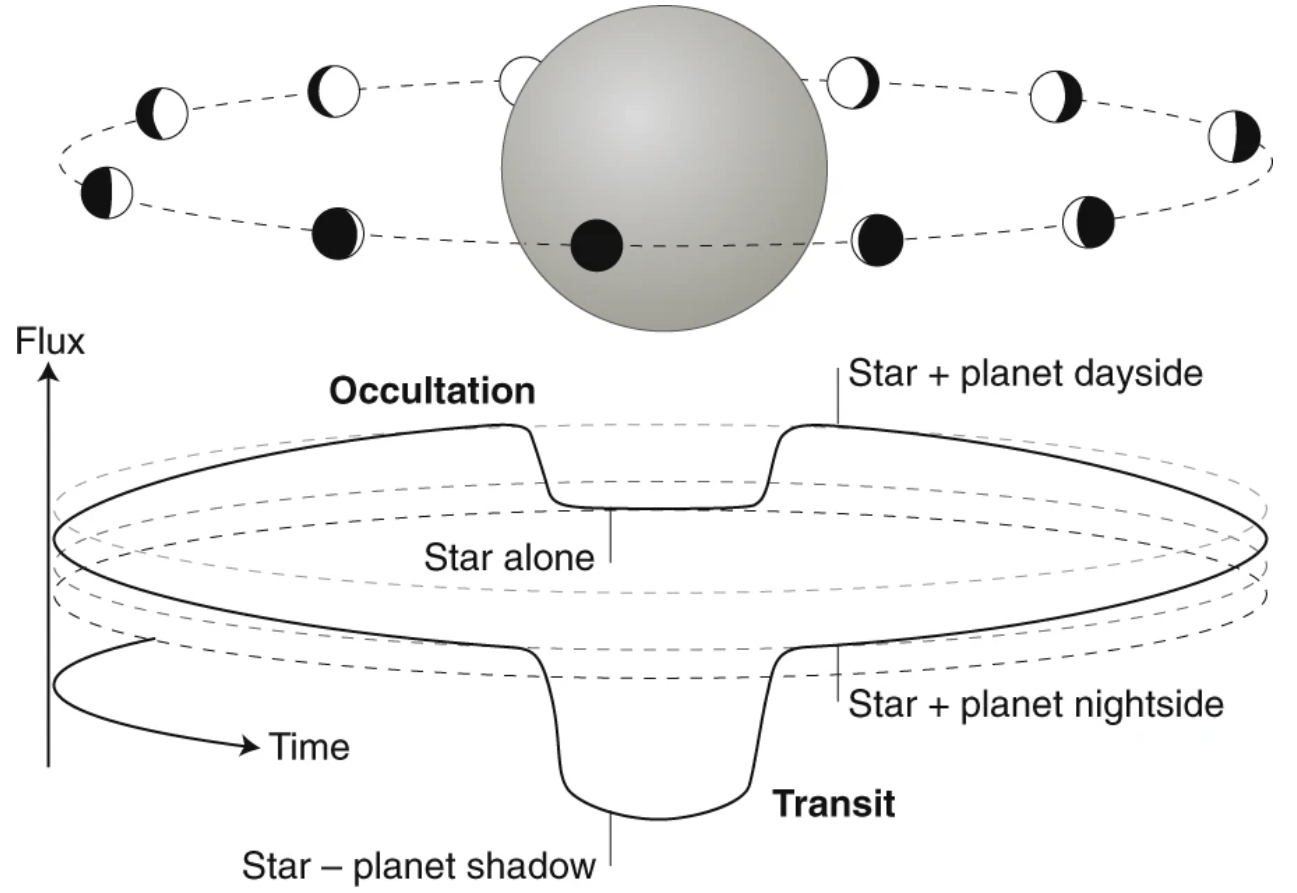
\includegraphics[width=0.75\textwidth]{transit.png}
		\caption{A qualitative illustration \cite{naturetransitfig} of the physical principle underlying the transit method. As the planet orbiting in the plane of sight, passes in front of its parent star, it eclipses the light from the star, resulting in a dip in the flux. If this dip is periodic the planet may be considered a planetary candidate. In addition, reflected light from the planetary surface will increase the flux slightly, and thus a secondary dip in the flux will be observed as the planet is eclipsed by the star. }
		\label{fig:transitmethod}
	\end{figure}
	One can detect an exoplanet and measure its size is via the so-called transit method. This method may be used if the orbit of the planet lies in the plane of sight. This method requires time-series measurements of small variations in the relative flux of a star. As the planet passes in front of its parent star, it eclipses the light from the star, and as a result, the flux is dimmed. By studying the relative flux of a star as a function of time, we may look for periodic dips in the flux indicating a possible planetary candidate. 
	
	The measured depth of the relative flux is approximated by $\delta$, the so-called \textbf{transit-depth} \cite{seagerintrotoexoplanets}
	\begin{equation}
		\Delta \bm F = \frac{\bm F(t)}{\bm F_s} \approxeq \left(\frac{R_\text{planet}}{R_\text{star}}\right)^2 = \delta,
	\end{equation}
	where $\bm F(t)$ is the temporal flux measured, $\bm F_s$ is the flux of the star when unobstructed, $R_\text{planet}$ is the radius of the potential planetary candidate and $R_\text{star}$ is the radius of the star. For an \textbf{earth-like} planet, around a sun-like star, this corresponds to measuring a depth of $84$ ppm \cite{cubesatexoplanet}. The transit method is illustrated in figure \ref{fig:transitmethod}.
	
	\section{Space mission requirements}
	When designing a space mission, such as STEP, mission requirements are defined. These requirements will ultimately determine the technical specifications of the spacecraft hardware. Requirements begin with well-defined user mission needs. In the case of the STEP mission, these needs are the scientific goals and requirements of the mission. Initially, the system is designed to meet these requirements while minimizing cost and risk. Often requirements defined from scientific goals will be ambitious and subject to requirements trading. Trading is the act of finding a compromise between what the user needs and what the buyer can afford \cite{SMAD}. For example, requirements may have to be loosened if the budget constrains the ability to meet the technical requirements that result from the mission requirements. In the present case of STEP, the scientific goal of performing photometry to a certain precision will directly impact the attitude and control subsystem of the satellite, as a high precision is reliant on very stable pointing abilities. The two requirements studied in this work will be derived and explained in detailed below.
	
	\section{The STEP mission design}
	In this section the relevant mission concepts are outlined. At first, the broad mission statement is presented. From this, the mission requirements that are investigated in this work will be established. 
	
	The STEP mission is a consortium of danish universities and the danish space industry \footnote{In particular STEP consists of \cite{stepprodex} Aarhus Universitet (AU), Danmarks Tekniske Universitet (DTU), Københavns Universitet (KU), Aalborg Universitet (AAU), Syddansk Universitet (SDU), DFM - Danmarks Nationale Metrologiinstitut, Terma Space, Space Inventor, GomSpace, SatLab and GateHouse Group}. STEP will supply chromatic time-series data of stars and exoplanets in the near UV range and visual parts of the electromagnetic spectrum. STEP will complement observational data from space- and ground telescopes; \footnote{TESS (NASA), Kepler (NASA), PLATO (ESA), James Webb Space Telescope (JWST; NASA and ESA), ARIEL (ESA), ESO and NOT}.
	
	To achieve these goals, the payload of the STEP mission will be a telescope with a CCD detector in the focal plane \cite{stepprodex}. 
	The delivered data will be photometric measurements of stars enabling the search for exoplanets via the transit method.
	
	The characteristics of the dip associated with the transit of an exoplanet in the near UV range will in complement to the same data in other parts of the spectrum, delivered by other telescopes mentioned above, enable the study of atmospheric properties of the planet. These atmospheric properties are phenomena such as cloud formation, atmospheric reflection and absorption, space weather, and the general impact on the evolution of exoplanets by their parent star. 
	
	% Please add the following required packages to your document preamble:
	% \usepackage[table,xcdraw]{xcolor}
	% If you use beamer only pass "xcolor=table" option, i.e. \documentclass[xcolor=table]{beamer}
	\begin{table}[]
		\centering
		\begin{tabular}{|l|}
			\hline
			\rowcolor[HTML]{C0C0C0} 
			\multicolumn{1}{|c|}{\cellcolor[HTML]{C0C0C0}\textbf{\begin{tabular}[c]{@{}c@{}}STEP\\ Mission objectives\end{tabular}}}                                                                                                                                                             \\ \hline
			\begin{tabular}[c]{@{}l@{}}\textbf{Primary objective:}\\ ~~\llap{\textbullet}~~ Provide extended time-series photometric observational data \\ \quad\; of stars in the near UV range, to search for exoplanets \\ \quad\;  and study their atmospheric properties.\end{tabular}                                              \\ \hline
			\begin{tabular}[c]{@{}l@{}}\textbf{Secondary objectives:}\\
				
				~~\llap{\textbullet}~~ To allow danish scientists and students to lead\\ \quad\; international research efforts in the field of stars and exoplanets \\
				~~\llap{\textbullet}~~ To strengthen the collaboration between universities\\ \quad\; and the space industries in Denmark \\
				
			\end{tabular} \\ \hline
		\end{tabular}
		\caption{A specification of the primary and secondary objectives of the STEP mission.}
		\label{table:missiongoals}
	\end{table}
	% Please add the following required packages to your document preamble:
	% \usepackage[table,xcdraw]{xcolor}
	% If you use beamer only pass "xcolor=table" option, i.e. \documentclass[xcolor=table]{beamer}
	\begin{table}[]
		\begin{tabular}{|ll|}
			\hline
			\rowcolor[HTML]{C0C0C0} 
			\multicolumn{2}{|c|}{\cellcolor[HTML]{C0C0C0}\textbf{\begin{tabular}[c]{@{}c@{}}STEP\\ Preliminary Top-level relevant Mission requirements\end{tabular}}}                                                                                                                                                                                       \\ \hline                                                      
			\rowcolor[HTML]{C0C0C0} 
			\multicolumn{1}{|l|}{\cellcolor[HTML]{C0C0C0}\textbf{Requirement}}                                    & \textbf{The STEP mission}                                                                                                                                                                                                                  \\ \hline
			
			\rowcolor[HTML]{C0C0C0} 
			\multicolumn{2}{|c|}{\cellcolor[HTML]{C0C0C0}\textbf{Functional}}                                                                                                                                                                                                                                                                      \\ \hline
			\multicolumn{1}{|l|}{Photometric Precision}                                                           & Knowledge of linearity curve to a precision of $5*10^{-4}$                                                                                                                                                                                                                      \\ \hline
			\multicolumn{1}{|l|}{\begin{tabular}[c]{@{}l@{}}Maximum differential flux\\ variability\end{tabular}} & \begin{tabular}[c]{@{}l@{}}Estimate allowed light centroid movement on CCD,\\ to constrain differential flux variabillity\\ due to movement to $1 \%$ of $1\% \;(10^{-4})$  \end{tabular}                                                                                                                                                                                                           \\ \hline
			\multicolumn{1}{|l|}{Secondary mission}                                                               & \begin{tabular}[c]{@{}l@{}}Detection of larger than earth sized planets\\ if cost constrains technical requirements\end{tabular}                                                                                           \\ \hline
			\rowcolor[HTML]{C0C0C0} 
			\multicolumn{2}{|c|}{\cellcolor[HTML]{C0C0C0}\textbf{Operational}}                                                                                                                                                                                                                                                                     \\ \hline
			\multicolumn{1}{|l|}{Duration}                                                                        & \begin{tabular}[c]{@{}l@{}}4 years nominal, \\ extended lifetime if technically feasible\end{tabular}                                                                                               \\ \hline
			\multicolumn{1}{|l|}{Data distribution}                                                               & \begin{tabular}[c]{@{}l@{}}Likely from local server after downlink\end{tabular}                                                                                                                                             \\ \hline
			\multicolumn{1}{|l|}{\begin{tabular}[c]{@{}l@{}}Data content,\\  form, and format\end{tabular}}       & \begin{tabular}[c]{@{}l@{}}FITS images of star field, in time series. \\ Specs depending on ADC and CCD/CMOS type used\end{tabular}                                                                                           \\ \hline
			\rowcolor[HTML]{C0C0C0} 
			\multicolumn{2}{|c|}{\cellcolor[HTML]{C0C0C0}\textbf{Constraints}}                                                                                                                                                                                                                                                                     \\ \hline
			\multicolumn{1}{|l|}{Initial schedule}                                                                        & \begin{tabular}[c]{@{}l@{}}\textbf{Preparations and concept} \\ Fall 2021\\ \textbf{Technical study} \\ January 2022 to June 2022\\ \textbf{Establishment/construction}\\ 1/7/2021 to 31/12/2025\\ \textbf{Operations} \\ 1/1/2026 - 1/1/2030\end{tabular} \\ \hline
			\multicolumn{1}{|l|}{Regulations}                                                                     & \begin{tabular}[c]{@{}l@{}}ESA Mission \\Support Danish research,  and space industries\end{tabular}                                                                                                                                       \\ \hline
		\end{tabular}
		\caption{The relevant technical specifications of the STEP mission.}
		\label{table:missionspecs}
	\end{table}
	
	\subsection{Quantitative mission needs and requirements}\label{sec:missobj}
	
	The two mission requirements studied in this work are the photometric precision\footnote{The photometric precision is the precision to which we measure stellar fluxes over time.} and attitude requirements\footnote{In simple terms, attitude requirements are the requirements posed on the pointing ability of the space telescope.}. In table \ref{table:missionspecs}, a quick outline of the relevant mission requirements is tabulated as suggested in \cite{SMAD}. These requirements are subject to requirements trading, a practice in which mission constraints may be loosened if the technical requirements that result from said mission requirements turn out to be too expensive, or infeasible in practice. 
	
	\subsubsection{Kepler HAT-P-7 precision findings as input for mission requirements}\label{sec:intromissionreqspecification}
	
	As an illustration of the importance of the characterization and testing procedure that is to be developed, an example may be drawn from the \textbf{Kepler mission}, from which we may also deduce the mission requirements. 
	The \textbf{Kepler Space Telescope} was a space mission launched from Cape Canaveral, Florida USA, on March 6th, 2009 \cite{keplerlaunch} into an Earth trailing heliocentric orbit. It is an example of an astronomical satellite mission to detect exoplanets. The telescope was designed with the goal of detection and not measurements of planetary sizes. Several thousands of exoplanets have been found using data from the Kepler telescope, mainly via the transit method \cite{planetarchive}. The Kepler payload consisted of a photometer constructed from an array of CCDs, much like the one that is to be flown on STEP. The CCD array can be seen in figure \ref{fig:keplerccd}. The Kepler mission will be used to derive the mission requirements for STEP. From this, input mission requirements may be obtained. 
	
	\begin{figure}
		\centering			
		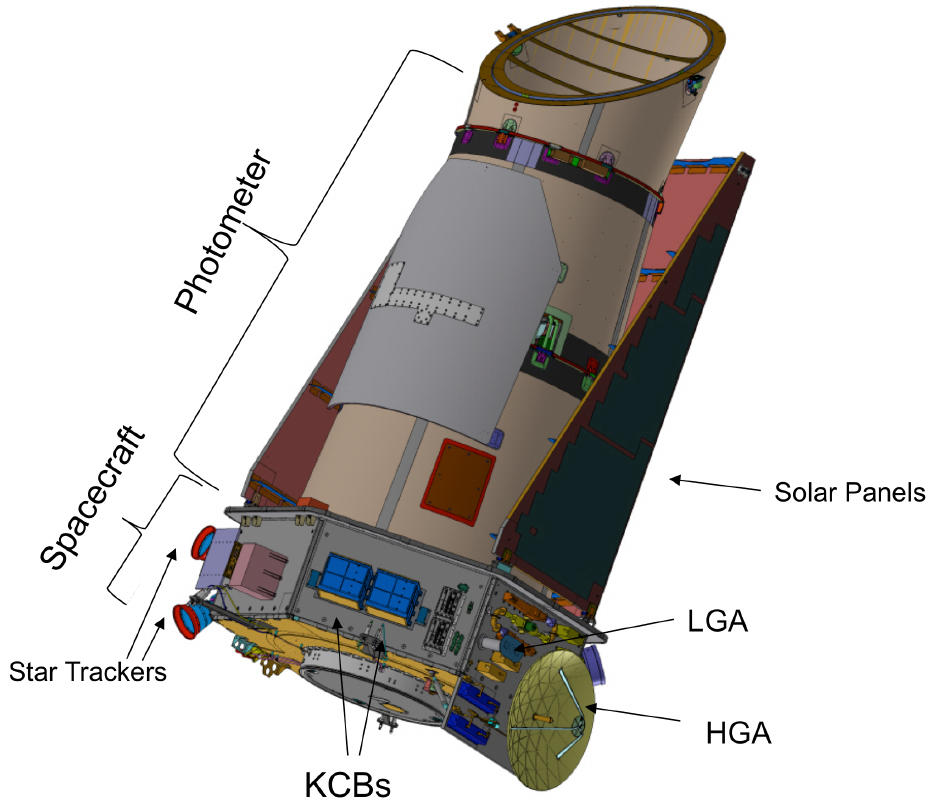
\includegraphics[width=.6\textwidth]{keplermodel.png}
		\caption{An illustration of the kepler spacecraft \cite{2016ksci.rept....1V}.}
		\label{fig:keplermodel}
	\end{figure} 
	
	One of the effects to be characterized is the CCD \textbf{linearity}. This will be explained in detail below (see section \ref{sec:linearity}). In short terms, it is a measure of how linear the response of the CCD is to changes in light intensities (or to the amount of light measured). Perfect linear behavior is when twice the number of 'counts' are measured when double the photons are incident on the detector. A CCD is in general not linear in this respect. This nonlinearity is probably due to the electronics in the detector, such as the amplification stage. It is also expected that if a light spot moves around on the detector, this will result in a change in the flux measured over time. This is because a CCD does not in general exhibit a linear and uniform response to light across the position on the detector. This is due to the way the detector is constructed. Channels of buried photoactive regions are constructed on the chip, and these make up the pixel columns. Movements may shine light onto the material in between the channels, and the photons are hence not detected. There may also be effects due to the way that the photoactive region of the CCD is constructed. Usually, CCDs are thinned by circular grinding, which may leave differences in the thickness of the photoactive material. A detailed discussion of how the CCD works and is built will be given in section \ref{sect:CCD}.
	
	\begin{figure}
		\centering			
		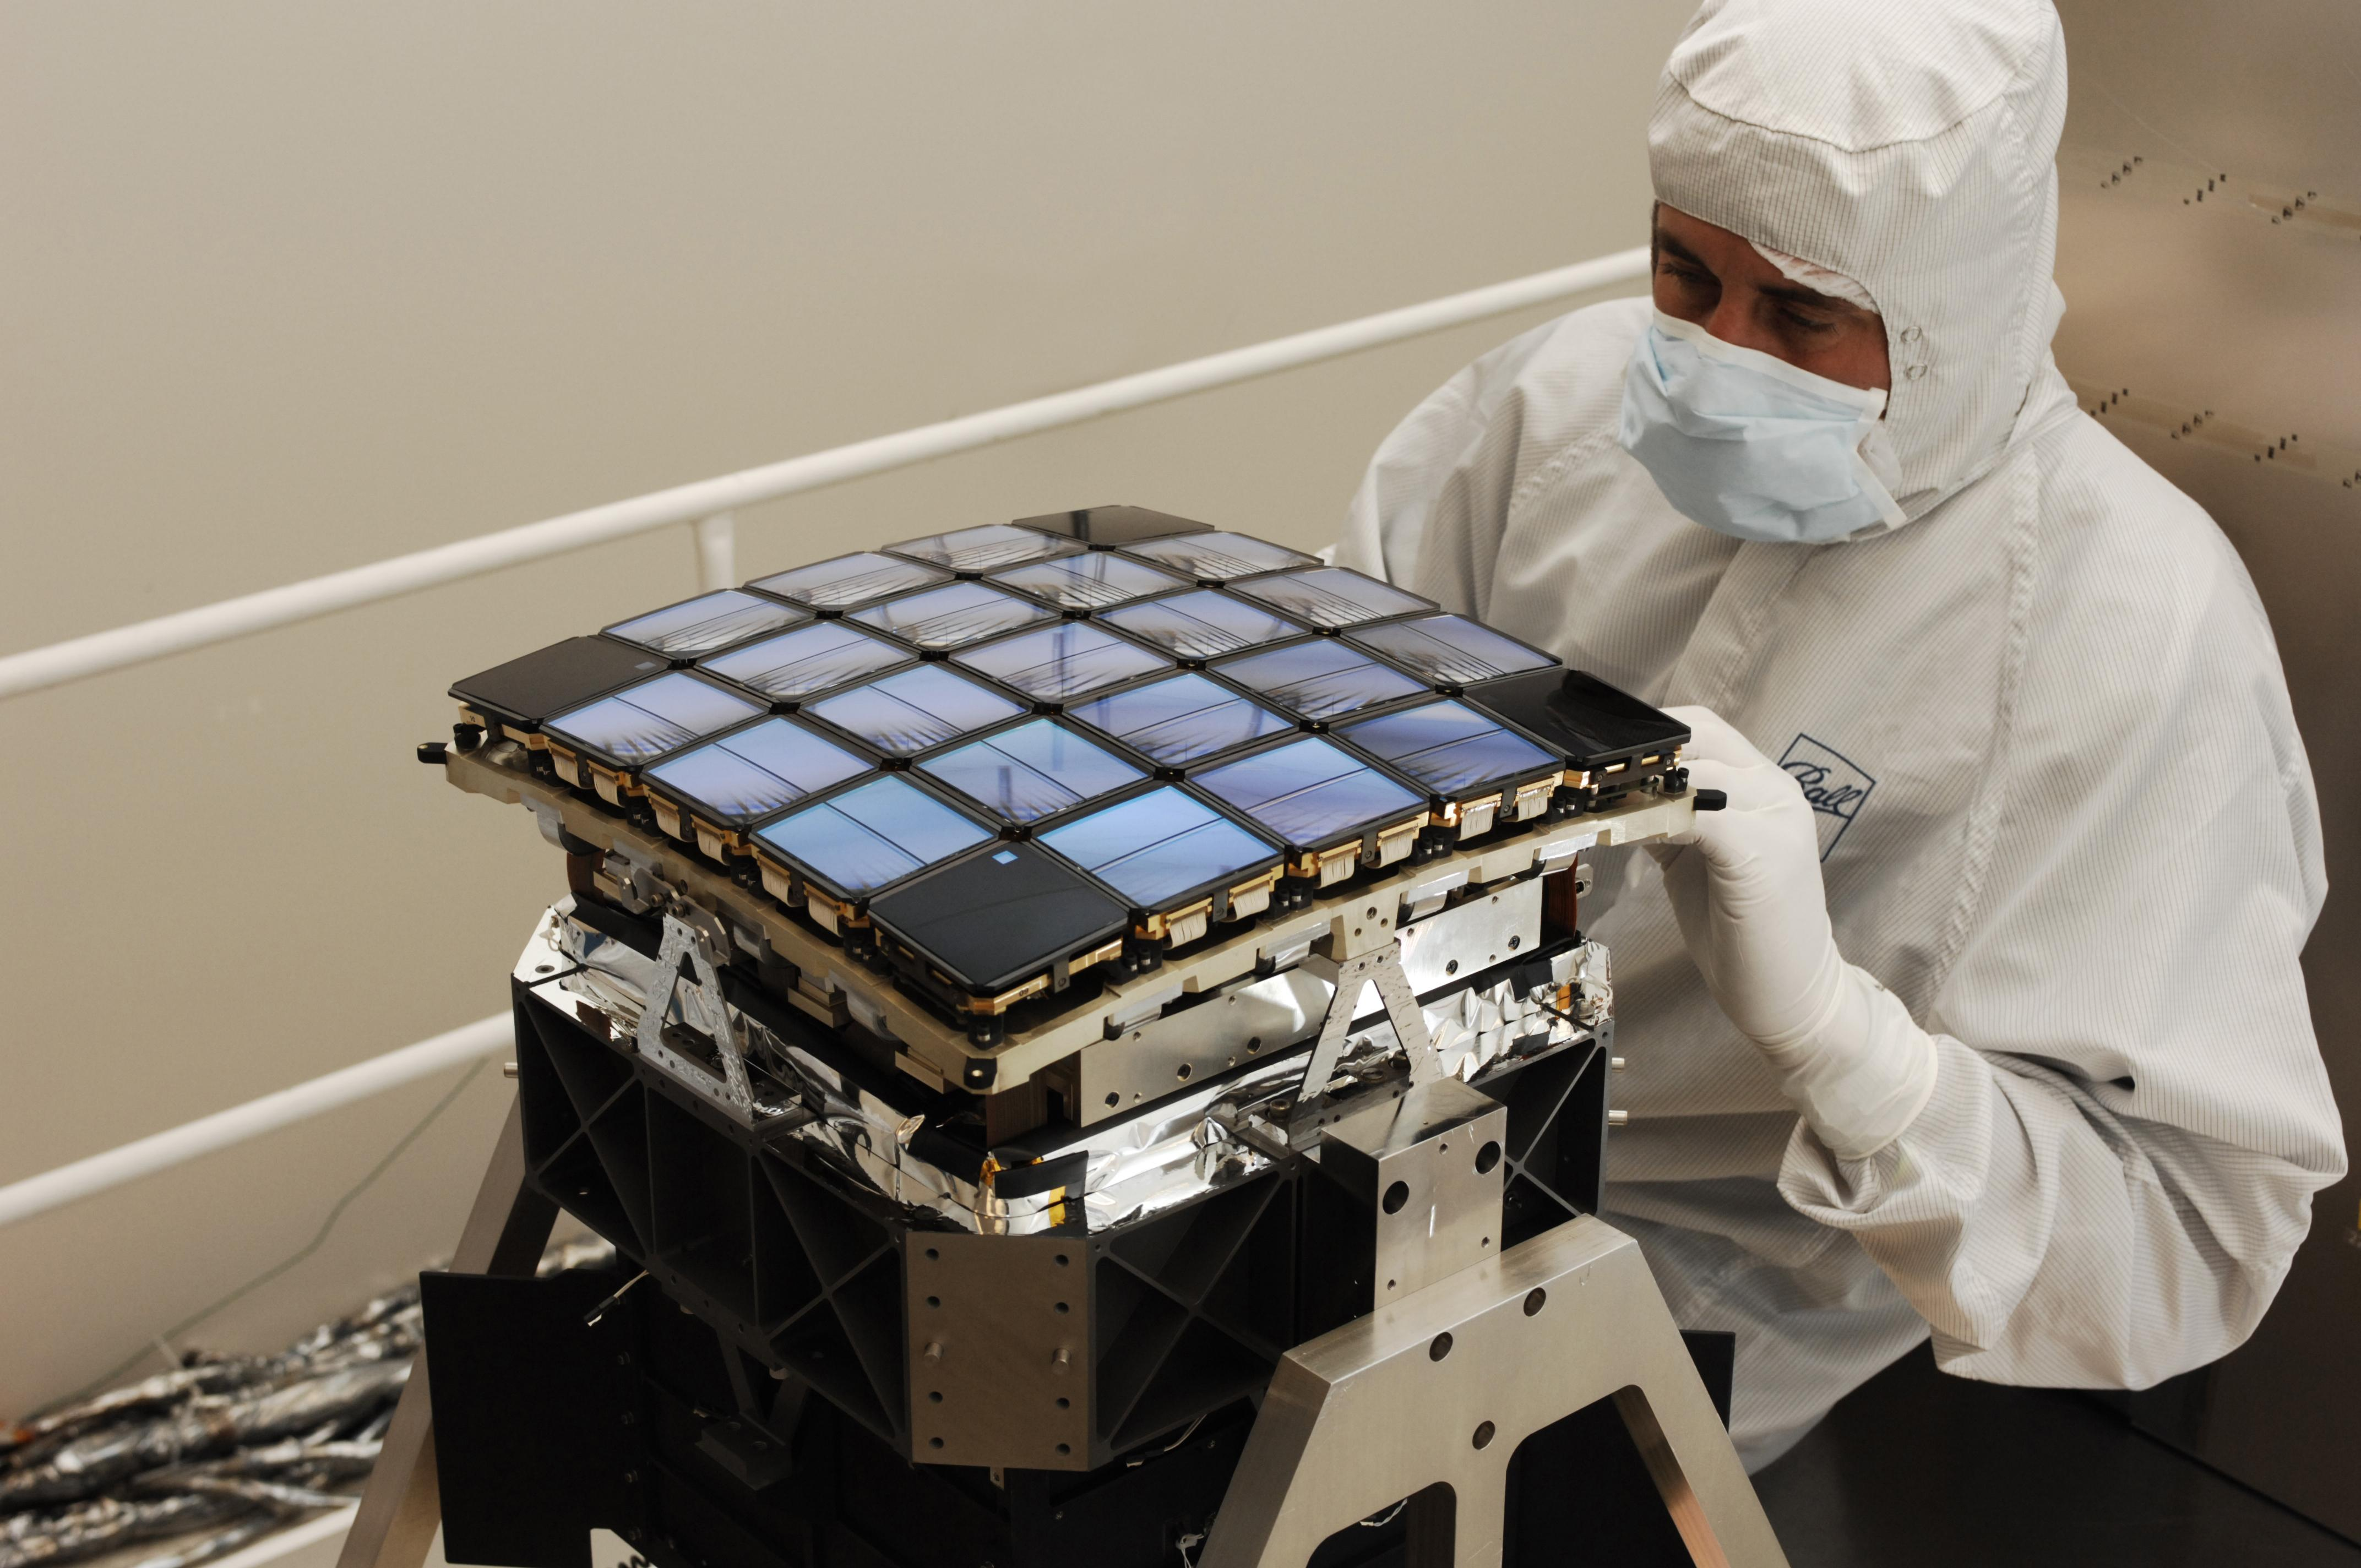
\includegraphics[width=1\textwidth]{keplerccd.jpg}
		\caption{A depiction \cite{keplerfocalplaneimage} of the Kepler focal plane consisting of an array of 42 charge coupled devices (CCDs).}
		\label{fig:keplerccd}
	\end{figure}
	
	The goal of the Kepler mission was exoplanet detection and not measurements of planetary sizes. Hence, a thorough construction of the linearity curve for each of the 42 CCDs was not carried out. The limits to the accuracy of Kepler planetary transit data have been studied in \cite{hatp7}, by observing systematic variations in transit depths of the \textbf{HAT-P-7} planetary system. 
	
	These effects are important to investigate since these flux changes could be misinterpreted as changes in the planetary system, perhaps due to a planetary transit. Kepler performed a quarterly $90^\circ$ roll, to realign solar panels towards the sun (from figure \ref{fig:keplermodel}, it is seen that the solar panels are on one side of the spacecraft), and hence some systematic effects are expected since the star will now be on a different detector (see figure \ref{fig:keplerccd}). The HAT-P-7 system is an ideal target for this analysis, as the star is bright with apparent magnitude $m_V = 10.5$\cite{hatp7}, and is orbited by a Hot Jupiter of radius $1.4 R_J$, with a short period of $2.2$ days. This results in frequent deep transits. These are determined from flux changes of the order of magnitude around $1\%$. 
	
	Two main systematic effects were observed by the authors. The first relates to the absolute measurement of the transit depth. This is related to both the pointing of the satellite, as well as the nonlinearity of the CCD. The authors concluded that transit depths vary on average as much as 1\% of the $1\%$ mean depth, between quarters. This is likely due to the nonlinearities of the instrument as the source illuminates a different part of the focal plane after a roll (hence is detected by a different CCD, which may have a different response altogether). This effect stems from movements on the focal plane. This can be due to different flux responses as the starlight moves around on the face of a single CCD, and hence constrains the pointing requirements of the satellite. It can also be due to differences in the response between flux levels, the nonlinearity of the detector. Due to these effects, the authors conclude that planetary radii cannot be estimated to a precision greater than 1\%, of the 1\% magnitude flux change that makes up the depth. Because of this, for STEP to do better than Kepler, and be able to measure planetary radii to the same precision, the first mission requirement may be stated as
	
	\begin{tcolorbox}[colframe = white, sharpish corners]
		\textbf{First mission requirement}
		\begin{quote}
			The attitude system should stabilize the pointing to such a degree that the flux does not vary by more than the order of magnitude of $10^{-4}$ or $0.01\%$. 
		\end{quote}
	\end{tcolorbox}
	
	The second systematic effect that was observed by the authors, is related to the precision in the differential measurement of the flux change. By considering a mean transit depth computed from the entire data set across all quarters, and mean transit depths computed from each of the four quarter types binned (so Q4-8-12 together, as well as Q1-5-9 and so on), a percentual depth difference may be computed. This is the second effect mentioned. These four 'differential' depths were found to have error bars of the order of magnitude of $5*10^{-4}$. With extensive knowledge of the linearity curve in each of the 42 detectors, changes due to varying responses to flux levels could likely have been corrected for, but only to the same precision of which the linearity curve is known (the errorbars on the linearity curve determine the precision). In the following, after the development of the characterization procedure, it shall be investigated whether it is feasible to construct the linearity curve to this precision. This gives us the second mission requirement stated as
	
	\begin{tcolorbox}[colframe = white, sharpish corners]
		\textbf{Second mission requirement}
		\begin{quote}
			The (non)linearity curve must be measured to a precision of at least $5*10^{-4}$.
		\end{quote}
	\end{tcolorbox}
	
	\subsection{Timeline and secondary missions}
	If it is infeasible to meet mission requirements, they may be loosened. This can result in new mission goals. Recently the STEP mission was subject to funding cuts which may alter the mission scope. The secondary missions arising from any subsequent requirements trading will most naturally be the search for planets with a size greater than Earth, as this poses lesser constraints on the hardware specifications. Larger planets give rise to deeper transit dips. Hence we may allow for a greater flux deviation while still being able to detect the transit. 
	Secondary missions can be stellar observations. These may be related to spectroscopy and asteroseismology. The former naturally requires a spectrometer, which may be a natural addition to the payload if feasible. The duration of the mission is set to be four years nominal with extension if allowed by the hardware. 
	
	\section{The desired end product and problem statement} 
	The end product desired from this work, is described in this section and consists of a detector characterization procedure and an attitude requirement test.
	
	The measurement of a transit depth is a differential measurement, and knowledge of the linearity curve will be crucial. Otherwise we can not know the actual depth of the transit. The linearity curve corrects for the nonlinearities in the data of the CCD flux response. It is used as a calibration yielding the actual flux. To construct this curve, a thorough characterization of the detector is necessary, and one of the goals of this work is to produce and verify such a characterization procedure. This procedure gives rise to a correction used to calibrate the detector, and the precision requirements pose constraints on the construction of the linearity curve.
	
	There will be variations in the flux due to small light spot movements on the detector plane. These changes will affect the measurement of the transit depth. A constraint on the allowable flux change directly results in a requirement on the satellite pointing stability. Thus, a test procedure to establish these attitude requirements from a constraint on the acceptable flux change will have to be designed. This test does not give rise to a correction scheme, but poses requirements on the satellite hardware.
	
	These considerations and the remarks of the preceding chapter lead to the following problem statement:
	\begin{tcolorbox}[colframe = white, sharpish corners]
		\textbf{Problem statement}
		\begin{quote}
			The goal of this work is to: 
			\begin{itemize}
				\item Describe the science case, and establish scientific mission requirements. 
				\item Account for and describe the physics of CCD detectors to design a CCD characterization procedure. 
				\item Verify the procedure and present it as an actionable measurement plan. 
				\item Characterize the CCD and compare the results to the scientific requirements. 
				\item Design a test procedure that will establish attitude requirements from scientific requirements. 
				\item Present a recommendation for future satellite missions.
			\end{itemize}
		\end{quote}
	\end{tcolorbox}
	\noindent The problem statement leads to the following structure of this text: The first part of the problem statement is accomplished in the present chapter. The science case was described, and the requirements were derived from the Kepler mission. In chapter 2, the physics of CCD detectors will be presented, beginning with the theory of solid-state photodetectors, and covering various physical effects in the detector. Chapter 3 presents the initial considerations regarding the characterization procedure, followed by the results and findings. A measurement plan is presented, and the calibration methods are described. In chapter 4, the problem of attitude control in photometry will be explained. Photometric methods and attitude control are described, followed by the experimental test design. Lastly, results and conclusions are presented. In chapter 5, the results and findings presented in this work are summarized and discussed. A discussion of prior satellite missions and their applied methods will be given, with the intention of a comparison to the present work. Finally, conclusions and recommendations for future missions will be given.
	
\end{document}